\chapter*{Copies of publications - Publikacijų kopijos}
\label{cha:publicationscopies} 
\addcontentsline{toc}{chapter}{\MakeUppercase{Copies of publications - Publikacijų kopijos}}
%% kai disertacija parengta mokslinių straipsnių rinkinio pagrindu)
%% Used, when you do not write a regular dissertation, you may need to include full papers in the dissertation
%% \parammarks{Copies of publications}


%  VU Leidykla paprašys prideti titulinį lapą prieš kiekvieną publikaciją. Kaip tai padaryti yra jusu pasirinkimas, bet galetu atrodyti taip:

\vspace*{15mm}

\begin{center}

{\huge 1st publication}
\vspace{10mm}

{\Large \bf Bare Demo of IEEEtran.cls for IEEE Journals}

\vspace{5mm}
\textbf{V. Pavardė}, V. Pavardė, and V. Pavardė

\vspace{5mm}
\textit{The Paper Title}, 24(5): 838--852, 2024


\vspace{3mm}
DOI: 10.15388/0.0.0.0

\end{center}

\newpage
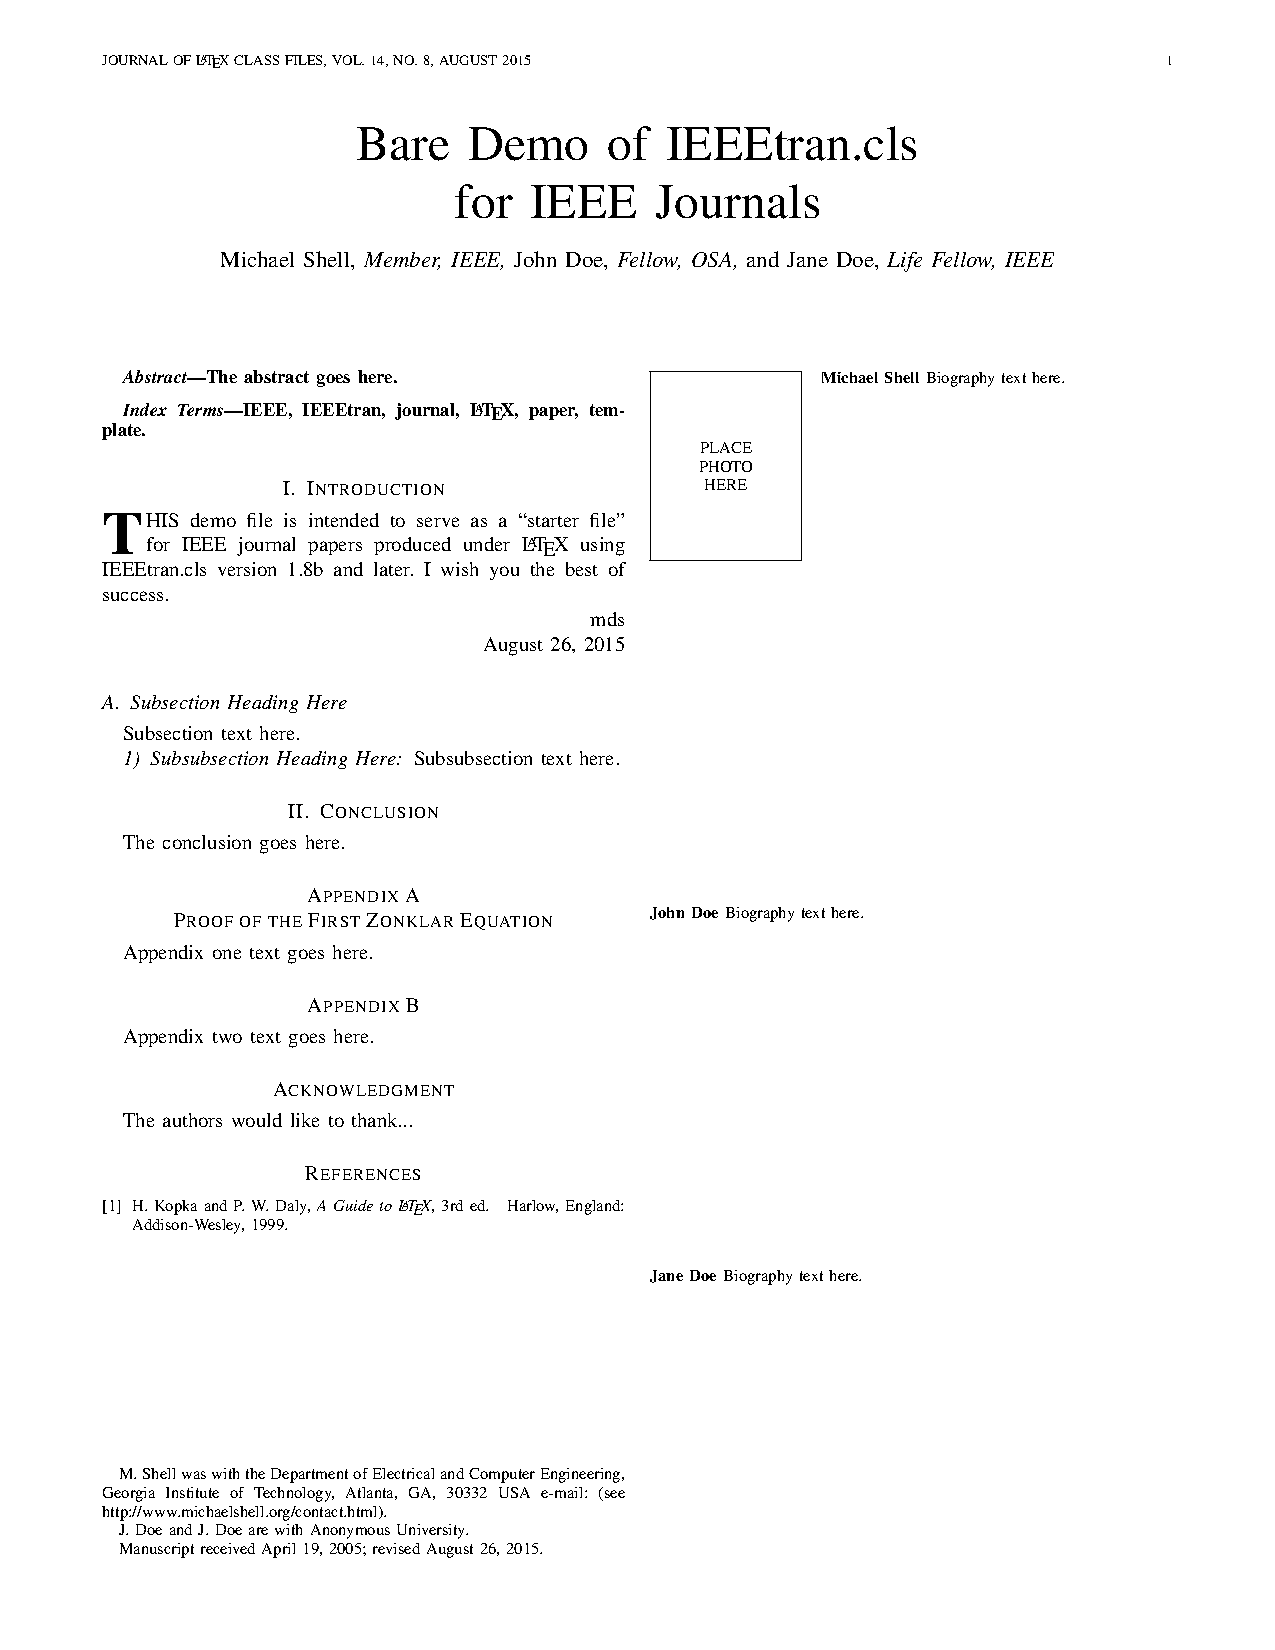
\includepdf[scale=1., pages=-]{"publications/author2024_publication_1.pdf"}